\pgfplotsset{compat=1.15}
\usetikzlibrary{arrows}
\definecolor{ududff}{rgb}{0.30196078431372547,0.30196078431372547,1}
\definecolor{qqffqq}{rgb}{0,1,0}
\definecolor{qqqqff}{rgb}{0,0,1}
\definecolor{ffqqqq}{rgb}{1,0,0}
\begin{figure}[h!]
\caption{Optimal solution for this instance of the \SPPN}
\centering
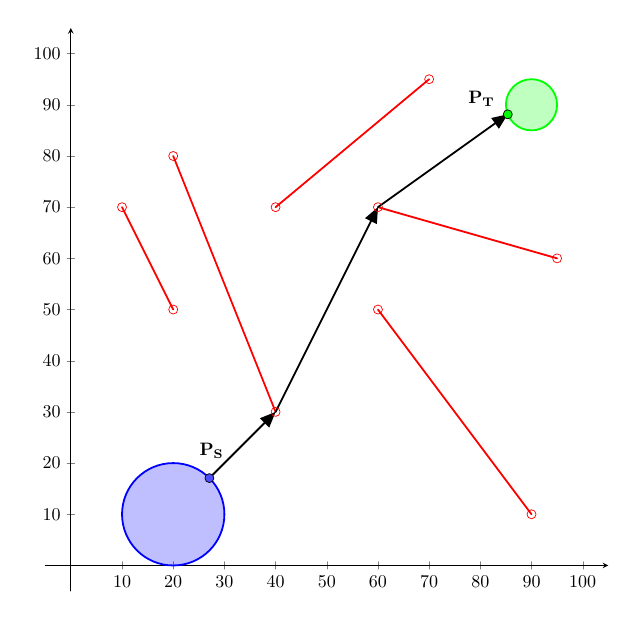
\begin{tikzpicture}[line cap=round,line join=round,>=triangle 45,x=1cm,y=1cm, scale=0.65]
\begin{axis}[
x=0.1cm,y=0.1cm,
axis lines=middle,
xmin=-5,
xmax=105,
ymin=-5,
ymax=105,
xtick={-30,-20,...,160},
ytick={-30,-20,...,95},]
\draw [line width=1pt,color=ffqqqq] (20,80)-- (40,30);
\draw [line width=1pt,color=ffqqqq] (70,95)-- (40,70);
\draw [line width=1pt,color=ffqqqq] (95,60)-- (60,70);
\draw [line width=1pt,color=ffqqqq] (60,50)-- (90,10);
\draw [line width=1pt,color=ffqqqq] (10,70)-- (20,50);
\draw [rotate around={0:(20,10)},line width=1pt,color=qqqqff,fill=qqqqff,fill opacity=0.25] (20,10) ellipse (1cm and 1cm);
\draw [rotate around={0:(90,90)},line width=1pt,color=qqffqq,fill=qqffqq,fill opacity=0.25] (90,90) ellipse (0.5cm and 0.5cm);
\draw [->,line width=1pt] (27.07,17.07) -- (40,30);
\draw [->,line width=1pt] (40,30) -- (60,70);
\draw [->,line width=1pt] (60,70) -- (85.36,88.14);
\draw (23.901825857302796,25.150339300103585) node[anchor=north west] {$\mathbf{P_S}$};
\draw (76.40719360287545,93.82231539794059) node[anchor=north west] {$\mathbf{P_T}$};
\begin{scriptsize}
\draw [color=ffqqqq] (20,80) circle (2.5pt);
\draw [color=ffqqqq] (40,30) circle (2.5pt);
\draw [color=ffqqqq] (70,95) circle (2.5pt);
\draw [color=ffqqqq] (40,70) circle (2.5pt);
\draw [color=ffqqqq] (95,60) circle (2.5pt);
\draw [color=ffqqqq] (60,70) circle (2.5pt);
\draw [color=ffqqqq] (60,50) circle (2.5pt);
\draw [color=ffqqqq] (90,10) circle (2.5pt);
\draw [color=ffqqqq] (10,70) circle (2.5pt);
\draw [color=ffqqqq] (20,50) circle (2.5pt);
\draw [fill=ududff] (27.07,17.07) circle (2.5pt);
\draw [fill=qqffqq] (85.36,88.14) circle (2.5pt);
\end{scriptsize}
\end{axis}
\end{tikzpicture}
\label{fig:solution_spp}
\end{figure}